% mnras_template.tex
%
% LaTeX template for creating an MNRAS paper
%
% v3.0 released 14 May 2015
% (version numbers match those of mnras.cls)
%
% Copyright (C) Royal Astronomical Society 2015
% Authors:
% Keith T. Smith (Royal Astronomical Society)

% Change log
%
% v3.0 May 2015
%    Renamed to match the new package name
%    Version number matches mnras.cls
%    A few minor tweaks to wording
% v1.0 September 2013
%    Beta testing only - never publicly released
%    First version: a simple (ish) template for creating an MNRAS paper

%%%%%%%%%%%%%%%%%%%%%%%%%%%%%%%%%%%%%%%%%%%%%%%%%%
% Basic setup. Most papers should leave these options alone.
\documentclass[a4paper,fleqn,usenatbib]{mnras}

% MNRAS is set in Times font. If you don't have this installed (most LaTeX
% installations will be fine) or prefer the old Computer Modern fonts, comment
% out the following line
\usepackage{newtxtext,newtxmath}
% Depending on your LaTeX fonts installation, you might get better results with one of these:
%\usepackage{mathptmx}
%\usepackage{txfonts}

% Use vector fonts, so it zooms properly in on-screen viewing software
% Don't change these lines unless you know what you are doing
\usepackage[T1]{fontenc}
\usepackage{ae,aecompl}


%%%%% AUTHORS - PLACE YOUR OWN PACKAGES HERE %%%%%

% Only include extra packages if you really need them. Common packages are:
\usepackage{graphicx}    % Including figure files
\usepackage{amsmath}    % Advanced maths commands
\usepackage{amssymb}    % Extra maths symbols

\usepackage{todonotes}
\graphicspath{{img/}}   % Set image path

%%%%%%%%%%%%%%%%%%%%%%%%%%%%%%%%%%%%%%%%%%%%%%%%%%

%%%%% AUTHORS - PLACE YOUR OWN COMMANDS HERE %%%%%

% Please keep new commands to a minimum, and use \newcommand not \def to avoid
% overwriting existing commands. Example:
%\newcommand{\pcm}{\,cm$^{-2}$}    % per cm-squared
\newcommand{\Sun}[0]{\ensuremath{_{\odot}}}
\renewcommand{\deg}{\ensuremath{^{\circ}}}


%%%%%%%%%%%%%%%%%%%%%%%%%%%%%%%%%%%%%%%%%%%%%%%%%%

%%%%%%%%%%%%%%%%%%% TITLE PAGE %%%%%%%%%%%%%%%%%%%

% Title of the paper, and the short title which is used in the headers.
% Keep the title short and informative.
\title[Auriga GCS]{The Globular Cluster System of the Auriga Simulations}

% The list of authors, and the short list which is used in the headers.
% If you need two or more lines of authors, add an extra line using \newauthor
\author[T. L. R. Halbesma et al.]{\parbox[t]{\textwidth}{
    Timo L. R. Halbesma$^{1}$\thanks{E-mail: Halbesma@MPA-Garching.MPG.DE},
    Wilma Trick$^{1}$,
    Robert J. J. Grand$^{1}$, 
    Volker Springel$^{1}$, 
    Facundo A. G\'{o}mez$^{2,3}$, 
    Federico Marinacci$^{4,5}$,
    R\"{u}diger Pakmor$^{1}$, 
    Simon D. M. White$^{1}$
} \vspace{10pt} \\
$^{1}$ Max-Planck-Institut f\"ur Astrophysik, Postfach 1317, D-85741 Garching, Germany \\
$^{2}$ Instituto de Investigaci\'{o}n Multidisciplinar en Ciencia yTecnolog\'{i}a, Universidad de La Serena, Ra\'{u}l Bitr\'{a}n 1305, La Serena, Chile \\
$^{3}$ Departamento de F\'{i}sica y Astronom\'{i}a, Universidad de La Serena, Av. Juan Cisternas 1200 N, La Serena, Chile \\
$^{4}$ Department of Physics, Kavli Institute for Astrophysics and Space Research, MIT, Cambridge, MA 02139, USA \\
$^{5}$ Harvard-Smithsonian Center for Astrophysics, 60 Garden Street, Cambridge, MA 02138, USA \\
}

% These dates will be filled out by the publisher
\date{Accepted XXX. Received YYY; in original form ZZZ}

% Enter the current year, for the copyright statements etc.
\pubyear{2019}

% Don't change these lines
\begin{document}
\label{firstpage}
\pagerange{\pageref{firstpage}--\pageref{lastpage}}
\maketitle

% Abstract of the paper
\begin{abstract}
We investigate whether the galaxy formation model used for the Auriga simulations 
can produce a realistic globular cluster population at redshift zero. We compare
properties of the simulated star particles in the Auriga haloes with
catalogues of observations of the Milky Way globular cluster population available
in the literature. We find that the Auriga simulations produce sufficient mass
at radii and metallicities that are typical for the MW GCS, although we observe
a varying mass-excess for the different $R_{\text{GC}}$-[Fe/H] bins. This implies
different values for the combined product of the bound cluster formation efficiency
and the globular cluster disruption rate. We investigate wether these differences
could result from formation insitu vs. accreted star particles. We find ...
\end{abstract}

% Select between one and six entries from the list of approved keywords.
% Don't make up new ones.
\begin{keywords}
methods: numerical -- galaxies: formation -- galaxies: star clusters: general.
\end{keywords}

%%%%%%%%%%%%%%%%%%%%%%%%%%%%%%%%%%%%%%%%%%%%%%%%%%

%%%%%%%%%%%%%%%%% BODY OF PAPER %%%%%%%%%%%%%%%%%%

\section{Introduction}
\todo[inline]{Paragraph: General introduction of GCs}

\citet{2005MNRAS.364..367D}: ``The radial profile of the stellar halo and metal-poor globular
clusters of the Milky Way suggest that these components formed in rare early peaks above $2.5 \sigma$ at redshift above 10. ''

\citet{2017MNRAS.465.3622R}: ``GCs among oldest astrophysical objects. GCs form in the early Universe in highest density peaks \citep[e.g.][]{2005MNRAS.364..367D, 2009ApJ...706L.192B}''




\begin{itemize}
    \item ``Hence, they witness most of the formation and evolution processes of galaxies, and can be used to probe them'' \citep{2006ARA&A..44..193B}
    \item ``colour bimodality, blue and red clusters \citep[e.g.][]{1985ApJ...293..424Z, 1999AJ....118.1526G, 2001AJ....121.2974L, 2006ApJ...639...95P}
    \item ``blue metal-poor (with distribution peaking at [Fe/H] $\approx -1.5$ for the Milky Way), no sign of rotation as a population (..) more metal-rich (peak at [Fe/H] $\approx -0.5$ in the Milky  Way) more spatially concentrated and rotating with the galaxy.'' \citep{1996AJ....112.1487H}
\end{itemize}
 
 


\todo[inline]{Paragraph: ``Bimodality suggests two formation mechanisms''. In-situ vs. Accreted}
\begin{itemize}
    \item ``Blue clusters from in early Universe in galaxies that merge later. In (wet) merger process starbursts generate red population \cite{1992ApJ...384...50A, 1987nngp.proc...18S}''
    \item ``\citet{1997AJ....113.1652F} propose instead that blue globulars form when the protogalaxy itself collapses, in a metal-poor and turbulence media. The red population would form later, once the galactic disc has settled. The formation of globular clusters would then be a multiphase process, with the first phase being interrupted possibly by cosmic reionization \citep{2002MNRAS.333..383B}.''
    \item ``\citet{2005ApJ...623..650K, 2014ApJ...796...10L} advocate
that major mergers are at the origin of both sub-populations: blue
clusters form during early mergers (z > 4) while the red ones appear
in mergers at lower redshifts (even after z = 1). Although, this
scenario, combined with star formation enhancement in mergers,
seems appropriate in dense galactic environment leading to the
assembly of massive elliptical galaxies, like in the Virgo Cluster
as tested by \citet{2014ApJ...796...10L}, it does not apply to Milky Way-
like systems where no recent major merger took place (Wyse 2001;
Deason et al. 2013; Ruchti et al. 2014, 2015).
\item ``\citet{1998ApJ...501..554C} argue that red clusters form in situ while the blue ones are accreted, either via merging satellite galaxies, or by tidal capture of the clusters themselves \citep[see also][]{2013ApJ...762...39T}.''
\end{itemize}


Dark Matter - GC connection

\todo[inline]{Paragraph: scientific motivation}
\begin{itemize}
    \item The star formation model implemented in the Auriga simulations is capable of producing a suite/population of realistic Milky Way-like galaxies at redshift zero.
    \item (However) State of the art simulations still face numerical restrictions that requires a subgrid approach to star formation and feedback because individual stars (and their evolution) cannot yet be accounted for. Star formation thus occurs in a heuristic/probabilistic fashion for gas cells that fulfill some star formation criterion. The star particles enrich the gas with metals and energy, both according to pre-defined/pre-calculated yields for specific feedback processes (supernova type I and II, strong stellar winds of asymptotic giant branch stars, ). In addition, black holes are seeded in eligible haloes to account for feedback associated with an active galactic nucleus.
    \item The end-result of the star formation model is the production of simulated Milky Way-like galaxies. Therefore the question naturally arises whether or not the Auriga simulations are also capable of faithfully producing a globular cluster population as observed in the Milky Way.
    \item Globular cluster formation in cosmological zoom simulations is very interesting for two reasons. First of all, extragalactic observations typically show the integrated properties of globular clusters rather than that of the individual stars within the clusters. Moreover, the typical mass scale of globular clusters is comparable to the numerical (mass) resolution of cosmological zoom simulations. The detailed small scale physics that is at play for real world globular clusters appears in observations as the combined effect of the $10^{3-6}$ M\Sun, compared to a mass resolution of $10^{3-5}$ M\Sun for the Auriga simulations. Globular clusters can therefore serve as an ultimate test to the star formation model that is implemented in the numerical simulations. Secondly, cosmological zoom simulations provide an accurate recording of the full and detailed merger history of the simulated galaxy. This is important because theoretical paradigms for globular cluster formation in the literature know two distinct classes of GCs that are separated by their exact formation sites: an in-situ versus an accreted population. Cosmological zoom simulations are uniquely allow for an investigation into globular cluster formation with particular focus on the in-situ and accreted populations.
\end{itemize}



\todo[inline]{Paragraph: previous work / work of other groups}
This goes before the GC formation mechanism paragraph.
\begin{itemize}
\item Origin of the Milky Way globular clusters \citep{2017MNRAS.465.3622R}
\item GCs in FIRE \citep{2018MNRAS.474.4232K}
\item EMOSAICS project \citep{2018MNRAS.475.4309P}
\item Origin of GC bimodality? \citep{2018MNRAS.479..200F}
\item \textit{GAIA} DR2: GC kinematics \citep{2018A&A...616A..12G}, Dating GC Tidal Disruption \citep{2018ApJ...859L..13B}
\item GC in N-body simulation \citep{2018ApJ...861...69C}
\item Tangentially related? role of GC mass evolution on stream properties \citep{2018MNRAS.474.2479B}
\item GC formation from dwarfs to giants \citep{2018MNRAS.480.2343C}
\item GC contribution to EOR \citep{2018MNRAS.479..332B}
\item Early Universe supermassive star / GC formation \citep{2018MNRAS.478.2461G}
\item GC formation in cold filaments \citep{2018ApJ...861..148M}
\item GC formation in high-redshift dwarf galaxies \citep{2018MNRAS.477..480Z}
\item GCs in MW outer region \citep{2017arXiv170804542P}
\item Impact of the Cutoff of the Cluster Initial Mass Function \citep{2018arXiv181001888C}
\item Metallicity gradients in the globular cluster systems of early-type galaxies: in situ and accreted components \citep{2018MNRAS.479.4760F}
\item Globular clusters in M31, Local Group, and external galaxies \citep{2016IAUS..317..120L}
\item Globular Clusters Formed within Dark Halos I: present-day abundance, distribution and kinematics \citep{2019MNRAS.482..219C}
\item The mass of the Milky Way from satellite dynamics \citep{2018arXiv180810456C}
\item Globular cluster formation and evolution in the context of cosmological galaxy assembly: open questions \citep{2018RSPSA.47470616F}
\item The kinematics of globular clusters systems in the outer halos of the Aquarius simulations \citep{2016A&A...592A..55V}
\item Star Cluster Formation in Cosmological Simulations \citep{2017ApJ...834...69L, 2018ApJ...861..107L, 2018arXiv181011036L}
\item A systematic analysis of star cluster disruption by tidal shocks -- I. Controlled N-body simulations and a new theoretical model \citep{2018arXiv181200014W}
\item Spatial mixing of binary stars in multiple-population globular clusters \citep{2018MNRAS.tmp.3147H}
\item Star Clusters Across Cosmic Time \citep{2018arXiv181201615K}
\item Kinematics of Subclusters in Star Cluster Complexes: Imprint of their Parental Molecular Clouds \citep{2018arXiv181201858F}
\item Investigating the population of Galactic star formation regions and star clusters within a Wide-Fast-Deep Coverage of the Galactic Plane  \citep{2018arXiv181203025P}
% TODO: last checked arXiv Dec 15, 2018
\end{itemize}


\todo[inline]{Paper outline}
We summarise the relevant characteristics of the Auriga simulations in section~\ref{sec:auriga}, followed by a summary of the observations of the Milky Way (MW) globular cluster system (GCS) in section~\ref{sec:observations} that we use to compare our simulations to in section~\ref{sec:results}. We discuss our findings in section~\ref{sec:discussion} to come to our conclusions in section~\ref{sec:conclusions}.


\section{The Auriga simulations}
\label{sec:auriga}
We use the Auriga \citep[][hereafter G17]{2017MNRAS.467..179G} simulations, a suite of high-resolution cosmological zoom simulations ran with a galaxy formation model that produces realistic Milky Way-like galaxies at redshift $z=0$. The simulations are performed with \textsc{arepo} \citep{2010MNRAS.401..791S, 2016MNRAS.455.1134P} that solves the magnetohydrodynamical equations on a moving mesh. See G17 for further details; here we briefly summarise the relevant properties.
\todo[inline]{Paragraph: Auriga boilerplate, paraphrased}

``The simulations include a comprehensive model for galaxy formation physics which includes important baryonic processes, such as

primordial and metal-line cooling \citep{2013MNRAS.436.3031V};

a sub-grid model for the interstellar medium that utilises an equation of state representing a two-phase medium in pressure equilibrium \citep{2003MNRAS.339..289S}
u
a model for the star formation and stellar feedback that includes a phenomenological wind model \citep{2014MNRAS.437.1750M, 2017MNRAS.467..179G}

and metal enrichment from SNII, SNIa and AGB stars \citep{2013MNRAS.436.3031V}

black hole formation and active galactic nucleus feedback (\citep{2005MNRAS.361..776S, 2014MNRAS.437.1750M, 2017MNRAS.467..179G}

a spatially uniform, time-varying UV background after reionization at redshift six \citep{2009ApJ...703.1416F, 2013MNRAS.436.3031V}

and magnetic fields \citep{2013MNRAS.432..176P, 2014ApJ...783L..20P}

The model was specifically developed for the \textsc{arepo} code and was calibrated to reproduce several observational results such as the stellar mass to halo mass relation, galaxy luminosity functions and the history of the cosmic star formation rate density.
''


\todo[inline]{What is the star formation density threshold?}
``The gas is assumed to be star-forming and thermally unstable for densities higher than a threshold density that we derive from the parameters of the two gas phases and the desired star formation time-scale to be $n = 0.13 \text{cm}^{-3}$.'' - \citep{2017MNRAS.467..179G}


\todo[inline]
``The diversity in morphological properties of these simulated galaxies reflects the stochasticity inherent to the process of galaxy formation and evolution \citep[e.g.][]{2005ApJ...635..931B, 2010MNRAS.406..744C, 2010ApJ...708.1398T}.''

\subsection{Definition of stellar halo}
\todo[inline]{Possibly also relevant here. See \citet{2018arXiv180407798M}.}


\subsection{Definition of accreted and in-situ component}
\todo[inline]{Possibly also relevant here. See \citet{2018arXiv180407798M}.}



\section{Relevant observational data for Local Group spirals}
The Milky Way + M31 globular cluster system
\label{sec:observations}

\subsection{Harris catalogue}
\label{sec:harris}
\citet[][2010 edition]{1996AJ....112.1487H} provides the most up-to-date and comprehensive catalog of the MW GCS that contains properties of 157 globular clusters. The catalogue is believed to be roughly 90\% complete.

\subsection{Age estimates}
\label{sec:vandenberg}
\citet{2013ApJ...775..134V} measured [Fe/H] and obtained age-estimates for 55 globular clusters in the MW GCS.


How is this particular sample selected? What biases does this introduce?
Is this sample drawn from the same underlying distribution as the Harris sample (plot distributions of FeH, compare mean/std, do t-test)

\subsection{M31}
\todo[inline]{Get big dataset of M31 GCS}
\label{sec:m31}
\citep{2011AJ....141...61C}
\citep{2014MNRAS.442.2165H, 2014MNRAS.442.2929V}




\section{Results}
\label{sec:results}
\citet{2013ApJ...775..134V} presents age measurements of 55 GCs in the MW. The
mean age of GCs in the MW is $11.9$~Gyr with a dispersion of $0.8$~Gyr. 
Therefore we select all star particles in the Auriga simulations that are older 
than $10$~Gyr. Henceforth we will refer the this subset of star particles as the 
`GC candidates'. Our approach is similar to the one taken by \citep{2017MNRAS.465.3622R},
where we know we are oversampling the real GC population with the contribution
of field stars in our subset. This will be further addressed in the discussion.

\subsection{Metallicity distribution}
\label{sec:metallicity}

Can the Auriga simulations produce star particles of $>10$~Gyr (GC candidates) with a metallicity distribution that is consistent with the MW GCS?

Fig.~\ref{fig:FeH}

Split into insitu / accreted


Conclusion: too many metal-rich star particles.


\begin{figure*}
    \includegraphics[width=\columnwidth]{{logMFeH_OldStars}.png}
    \includegraphics[width=\columnwidth]{{logMFeH}.png}
\end{figure*}
\begin{figure*}
    \includegraphics[width=\columnwidth]{{logMFeH_OldInsitu}.png}
    \includegraphics[width=\columnwidth]{{logMFeH_OldAccreted}.png}
    \caption{Caption}
    \label{fig:FeH}
\end{figure*}



\subsection{Spatial distribution}
\label{sec:spatial}
Is the spatial distribution of the GC candidates in the Auriga simulations consistent with the MW GCS?


Look into Pandromeda survey? Star counts, very wide angle survey

\begin{figure*}
    \includegraphics[width=\columnwidth]{{logMRgc_OldStars}.png}
    \includegraphics[width=\columnwidth]{{logMRgc}.png}
\end{figure*}
\begin{figure*}
    \includegraphics[width=\columnwidth]{{logMRgc_OldInsitu}.png}
    \includegraphics[width=\columnwidth]{{logMRgc_OldAccreted}.png}
    \caption{Caption}
    \label{fig:Rgc}
\end{figure*}



\subsection{Age-metallicity distribution}
\label{sec:agemetallicity}
What age-metallicity distribution is produced by star formation events in the Auriga simulations?



\subsection{Mass budget} 
\label{sec:mass}
Does the star formation model implemented in the Auriga simulations produce sufficient mass in star particles with properties that are consistent with the MW GCS?

What efficiencies could we afford if we would take into account the combined mass loss effect of converting from star particles to bound star clusters and globular cluster disruption?

How does the total stellar mass in $R_\textbf{GC}$-[Fe/H] bins compare to the MW GCS?



\subsection{Formation history} 
\label{sec:history}
Can we identify particular star formation events that generate GC candidates with the correct age, metallicity, and radial properties as expected or the MW GCS?

Can we distinguish between particles that have formed in-situ and those that have been accreted? Can we identify specific features in the age-metallicity plane, or in the $R_\textbf{GC}$-[Fe/H] plane, that result from one of both populations? How does this connect to proposed mechanisms for globular cluster formation in the literature?


Orbits: are the pericentres different? Look at velocity + specific angular momentum distribution in the different FeH/Rgc bins as proxy for the pericenter




\subsection{Scatter for different Auriga haloes} 
\label{sec:convergence}
Are the properties of the Auriga globular cluster candidates converged for runs with different initial conditions but at the same resolution level? How much scatter do we observe in the properties of the globular cluster candidates across the full suite of Auriga haloes?



\subsection{Numerical convergence (possibly in appendix)} 
\label{sec:convergence}
Are the properties of the Auriga globular cluster candidates converged for runs with the same initial conditions but at different resolution levels? 

\begin{figure*}
    \includegraphics[width=0.31\textwidth]{{logMFeH_Au6}.png}
    \includegraphics[width=0.31\textwidth]{{logMFeH_Au16}.png}
    \includegraphics[width=0.31\textwidth]{{logMFeH_Au24}.png}
    \caption{Caption}
    \label{fig:FeH_l345}
\end{figure*}
\begin{figure*}
    \includegraphics[width=0.31\textwidth]{{logMRgc_Au6}.png}
    \includegraphics[width=0.31\textwidth]{{logMRgc_Au16}.png}
    \includegraphics[width=0.31\textwidth]{{logMRgc_Au24}.png}
    \caption{Caption}
    \label{fig:Rgc_l345}
\end{figure*}






% \begin{figure*}
%     \includegraphics[width=\textwidth]{{Au4-24_GCS_250_10}.pdf}
%     \caption{TODO: combine upper left and mid left panel, remove upper right panel,
%              remove lower panels (because mid right panel already shows the 
%              relevant info). The point of this figure is to compare metallicity 
%              distribution and radial distribution}
%     \label{fig:FeH_Rcs_MWvsAu424_1D}
% \end{figure*}
% 
% 
% \begin{figure*}
%     \includegraphics[width=\textwidth]{{Au4-24_FeH_vs_Rgc}.pdf}
%     \caption{Comparison of [Fe/H] and galactocentric radius of the Milky Way GCS
%              (red dots) with the star particles in Au4-24. TODO: only show the
%              panel on the right-hand side. TODO: include details of exactly which
%              star particles are shown. TODO: generate the same figure but color-coded
%              by mass?}
%     \label{fig:FeH_Rcs_MWvsAu424_2D}
% \end{figure*}
% 
% 
% \begin{figure*}
%     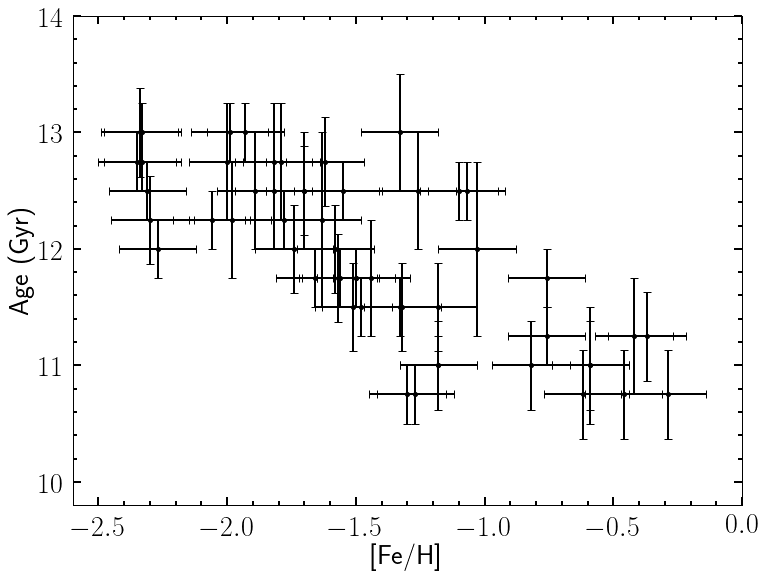
\includegraphics[width=\columnwidth]{vandenBergh2013.png}
%     \includegraphics[width=\columnwidth]{{Au4-24_Renaud2017_figure8}.png}
%     \caption{TODO: add observed age-FeH data points \citep{2013ApJ...775..134V}
%              to simulation plot, investigate starbursts by making pictures of
%              these events, check if the observed data set shows a representative
%              sample of the MW GCS, fix overlapping axes labels}
%     \label{fig:bla}
% \end{figure*}
% \begin{figure}
%     \includegraphics[width=\columnwidth]{{Au4-24_Renaud2017_figure6}.png}
%     \caption{}
%     \label{fig:bla}
% \end{figure}






\section{Discussion}
\label{sec:discussion}


\section{Summary and conclusions}
\label{sec:conclusions}


\section*{Acknowledgements}
TLRH acknowledges support from the International Max-Planck Research School (IMPRS) on Astrophysics.

\todo[inline]{Check Auriga boilerplate that we need to acknowledge}
RG and VS acknowledge support by the DFG Research Centre SFB-881 `The
Milky Way System' through project A1. This work has also been
supported by the European Research Council under ERC-StG grant
EXAGAL- 308037. Part of the simulations of this paper used the
SuperMUC system at the Leibniz Computing Centre, Garching,
under the project PR85JE of the Gauss Centre for Supercomputing.
This work used the DiRAC Data Centric system at Durham
University, operated by the Institute for Computational Cosmology
on behalf of the STFC DiRAC HPC Facility `www.dirac.ac.uk'.
This equipment was funded by BIS National E-infrastructure capital 
grant ST/K00042X/1, STFC capital grant ST/H008519/1 and
STFC DiRAC Operations grant ST/K003267/1 and Durham University. 
DiRAC is part of the UK National E-Infrastructure.

%%%%%%%%%%%%%%%%%%%%%%%%%%%%%%%%%%%%%%%%%%%%%%%%%%

%%%%%%%%%%%%%%%%%%%% REFERENCES %%%%%%%%%%%%%%%%%%

% The best way to enter references is to use BibTeX:

\bibliographystyle{mnras}
\bibliography{AurigaGCS} % if your bibtex file is called example.bib


% Alternatively you could enter them by hand, like this:
% This method is tedious and prone to error if you have lots of references
%\begin{thebibliography}{99}
%\bibitem[\protect\citeauthoryear{Author}{2012}]{Author2012}
%Author A.~N., 2013, Journal of Improbable Astronomy, 1, 1
%\bibitem[\protect\citeauthoryear{Others}{2013}]{Others2013}
%Others S., 2012, Journal of Interesting Stuff, 17, 198
%\end{thebibliography}

%%%%%%%%%%%%%%%%%%%%%%%%%%%%%%%%%%%%%%%%%%%%%%%%%%

%%%%%%%%%%%%%%%%% APPENDICES %%%%%%%%%%%%%%%%%%%%%

\appendix

\section{Some extra material}

If you want to present additional material which would interrupt the flow of the main paper,
it can be placed in an Appendix which appears after the list of references.

%%%%%%%%%%%%%%%%%%%%%%%%%%%%%%%%%%%%%%%%%%%%%%%%%%


% Don't change these lines
\bsp    % typesetting comment
\label{lastpage}
\end{document}

% End of mnras_template.tex
